\begin{appendices}
\section {Pileup rejection with R3B MUSIC charge cut}\label{app:r3bmusic_pileup}

As detailed in Section~\ref{subsec:event-sel}, a stringent event selection criterion was applied to the incoming ions. This included a precise charge cut, as illustrated in Figure~\ref{fig:r3bmusic_charge}. The application of a rigid $\pm 1 \sigma$ charge cut, in conjunction with the requirement of a single hit in the Start detector, effectively suppresses pileup events. The superior pileup rejection capability of the R3B MUSIC detector, owing to its longer shaping time compared to the TWIN MUSIC detector, is further demonstrated in Figure~\ref{fig:r3b_vs_twin_charge_def}. This extended shaping time ensures that any genuine pileup event will be reliably registered by the R3B MUSIC.
\begin{figure}[htpb]
    \centering
    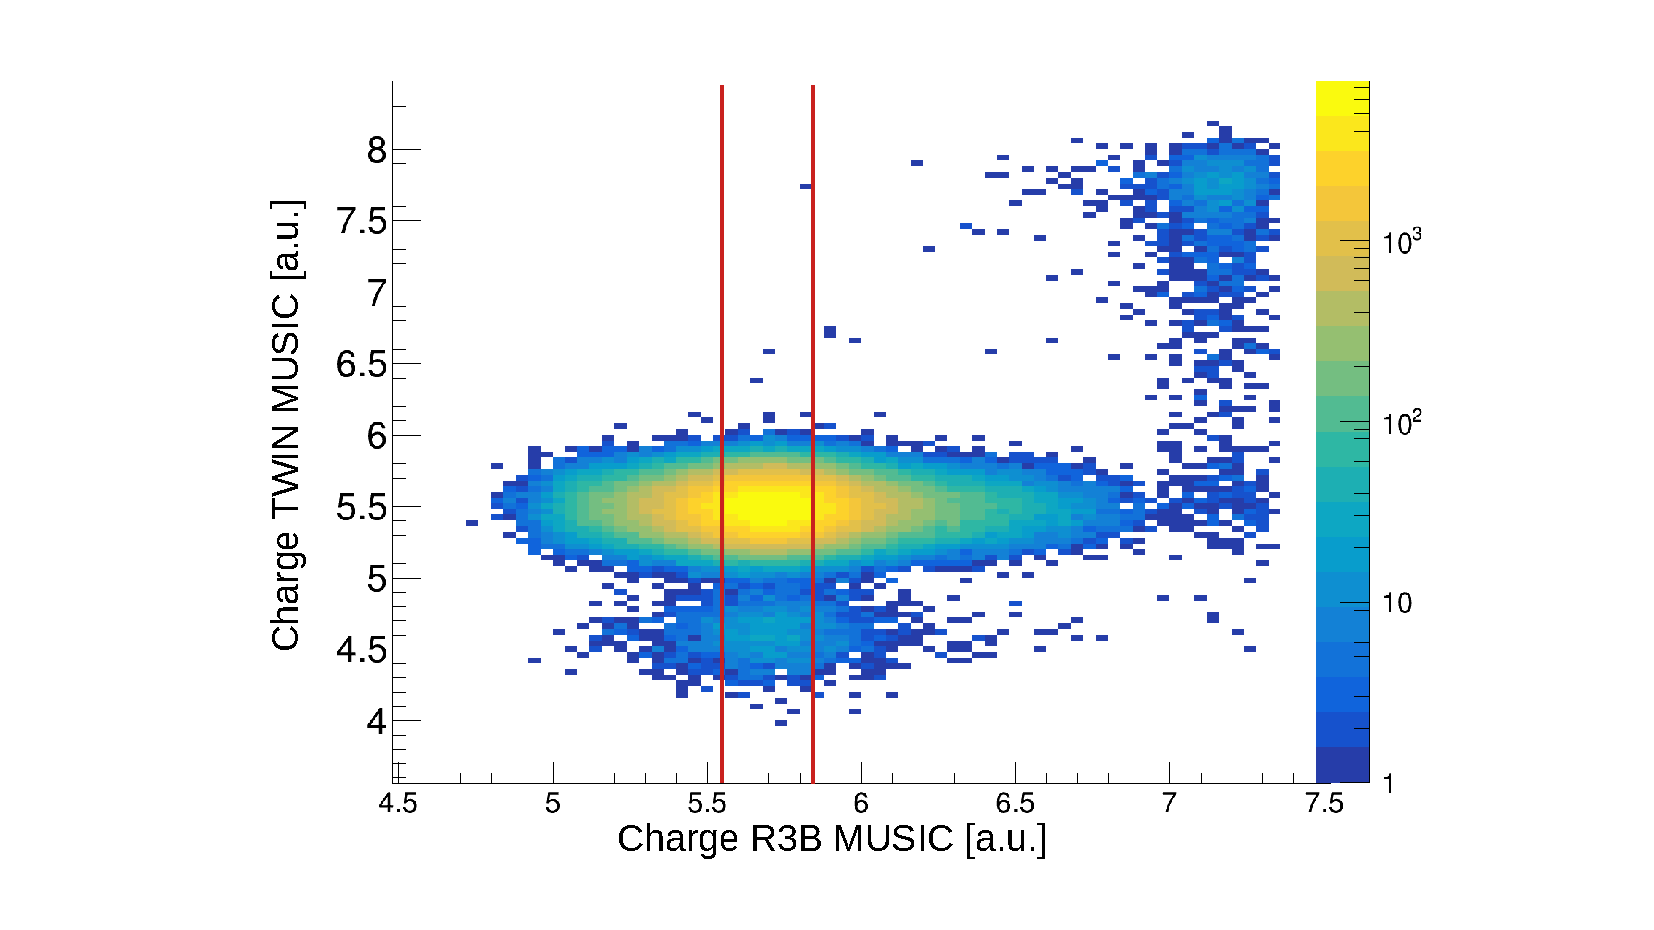
\includegraphics[width=\textwidth,keepaspectratio=true]{Figures/app_charge_r3b_twin_default.pdf}
    \caption{
	Charge distribution in R3B MUSIC vs TWIN MUSIC. The strict charge cut -- only events within the two horizontal lines are selected for the analysis -- on R3B MUSIC fully supresses pileup events. For this plot positional cuts on the MWPC0  and the requirement of a single hit in the Start detector are applied. Target run, 550 AMeV. 
    }
    \label{fig:r3b_vs_twin_charge_def}
\end{figure}

\section {MWPCs - \textit{cal-to-hit} data processing}


For all MWPCs the standard  \textit{cal-to-hit} step  sorts the calibrated hits in the detector according to the calibrated charge deposited in the pads. The final position (in mm) is determined by selecting the hit with the highest charge deposition $Q_{max}$ and its left ($Q_L$) and right neighbor ($Q_R$) pads\footnote{In case no charge deposition in one or both neighbors the charge value is set to 1 respectively.}. These charge and position values are inserted in the "hyperbolic squared secant" function \cite{lau1995optimization} with the following charge distribution function:
\[
Q(x) = \frac{a_1}{\cosh^2\left(\frac{\pi (x - a_2)}{a_3}\right)}
\]
\vspace{-0.5em} % Reduces the space between equations
where \(a_1\) is the amplitude of the distribution $Q_{max}$, \(a_2\) its centroid, and \(a_3\) derives as follows:
\[
a_3 = \frac{\pi \omega}{\cosh^{-1}\left(0.5 \times \left(\sqrt{\frac{Q_{\text{max}}}{Q_L}} + \sqrt{\frac{Q_{\text{max}}}{Q_R}}\right)\right)}
\]
\vspace{-0.5em} % Reduces the space between equations
\(\omega\) being the width of the pads. The centroid of the distribution, which is used as final hit position in the \textit{hit-}data level, can be deduced from:
\vspace{-0.5em} % Reduces the space between equations
\[
a_2 = \frac{a_3}{\pi} \times \tanh^{-1}\left(\frac{\sqrt{\frac{Q_{\text{max}}}{Q_L}} - \sqrt{\frac{Q_{\text{max}}}{Q_R}}}{2 \sinh\left(\frac{\pi \omega}{a_3}\right)}\right)
\]
Figure \ref{fig:hyp_function} shows the "hyperbolic squared secant" function with the inserted values for $Q_{max}$, $Q_R$ and $Q_L$. 
\begin{figure}[htpb]
    \centering
    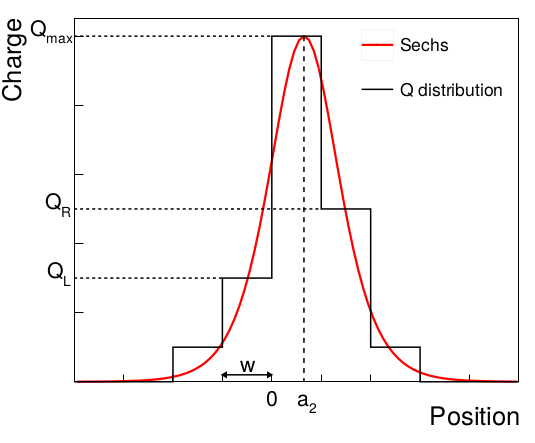
\includegraphics[width=\textwidth,height=8cm,keepaspectratio=true]{Figures/hyperbolic_squared_secant_function.png}
    \caption{
   	 Figure taken from \cite{martin2021fission}, with w being the with of the cathode pads of the MWPC and $a_2$ the final position value of the hit determined by the hyperbolic squared secant function (in red). In black the measured charge deposition distribution in the MWPC. 
     }
    \label{fig:hyp_function}
\end{figure}
The "hyperbolic squared secant" function is used to determine the x hit position as well as the y hit position for all MWPCs. Figure \ref{fig:x_mw23_default} shows the $x_{mw2}$ versus $x_{mw3}$ distribution of carbon isotopes for the 400 AMeV run with the thick target. The two correlated lines corresponding to the $^{12}$C and $^{11}$C isotopes can clearly be distinguished. The vertical line can be interpreted as amount of events where the incoming centered carbon fragment gets scattered by air or the detector material in place between MWPC2 and MWPC3. The horizontal wide spread line has no physical interpretation and can rather be explained by the \textit{cal-to-hit} step in MWPC2: For events where there is not a spatially constrained hit cluster but sparse hits the hyperbolic squared secant function may pick the wrong $Q_{max}$ and therefore wrongly reconstructs the x position in MWPC2. 
\begin{figure}[htpb]
    \centering
    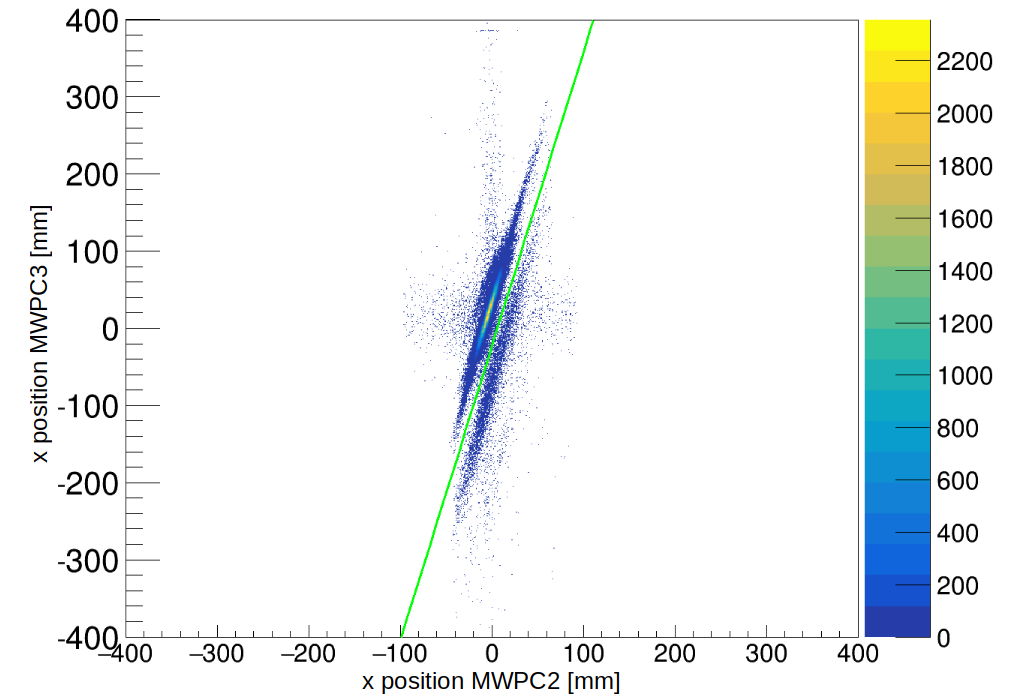
\includegraphics[width=\textwidth,height=8cm,keepaspectratio=true]{Figures/mw23_default.png}
    \caption{
   	 Distribution of x in MWPC2 and MWPC3 for the 400 AMeV run with thick target. The green line acts as reference line for the isotope separation between $^{12}$C and $^{11}$C/$^{10}$C.
     }
    \label{fig:x_mw23_default}
\end{figure}


\subsection {Coherent clustering} 

To overcome the issue with potentially wrong x- or y-position reconstruction in the MWPCs the event selection can be restricted to events where the MWPCs of interest have only one spatially constrained cluster(see figure \ref{fig:own_clustering}) to avoid ambiguities in the position determination.\newline
\begin{figure}
\floatbox[{\capbeside\thisfloatsetup{capbesideposition={left,top},capbesidewidth=6cm}}]{figure}[\FBwidth]
{\caption{Restricted event selection for MWPC2 and MWPC3: only events with one single coherent (i.e. without any holes) cluster are accepted.}\label{fig:own_clustering}}
{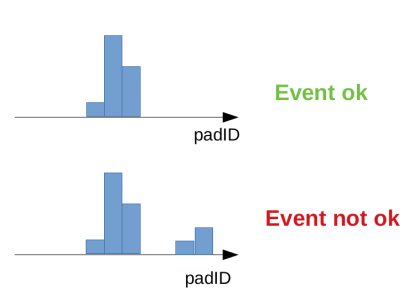
\includegraphics[width=7cm]{Figures/own_clustering_mwpcs.png}}
\end{figure}
Figure \ref{fig:mw23_own_clustering} shows the distribution of x in MWPC2 and MWPC3 using the coherent clustering reconstruction. This reconstruction method removes the uncorrelated horizontal line which was observed in figure \ref{fig:x_mw23_default}. However the statistics are reduced by approximately $35\%$\footnote{Number of entries in the 2D plot for default reconstruction method: 533816, for the coherent clustering reconstruction: 346315 for the 400 AMeV run with thick target.}.
\begin{figure}[htpb]
    \centering
    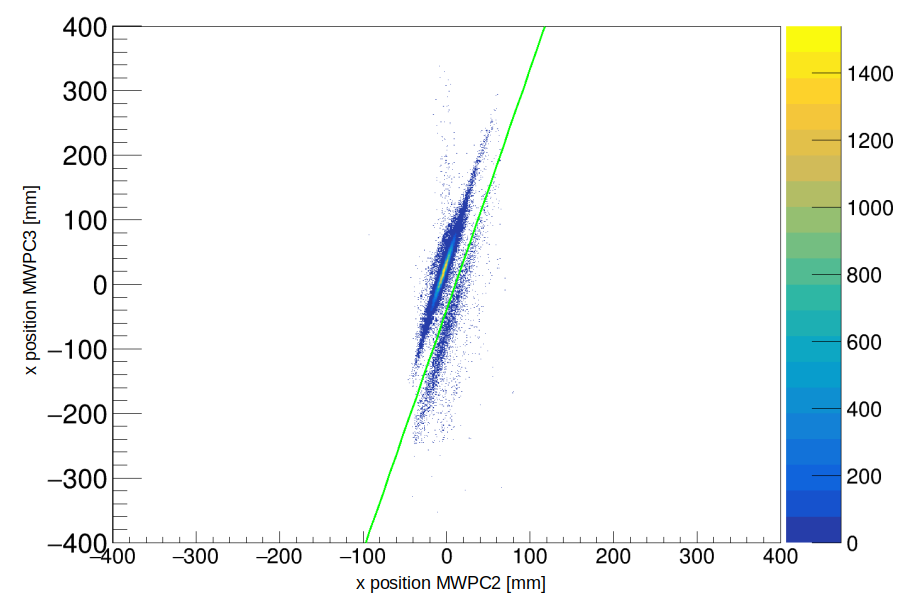
\includegraphics[width=\textwidth,height=8cm,keepaspectratio=true]{Figures/mw23_own_clustering.png}
    \caption{
   	 Distribution of x in MWPC2 and MWPC3 using the coherent clustering reconstruction. Thick target run, beam energy 400 AMeV. The green line acts as reference line for the isotope separation between $^{12}$C and $^{11}$C/$^{10}$C.
     }
    \label{fig:mw23_own_clustering}
\end{figure}

\section {MWPC0 selection cuts}\label{app:mw0_cuts}

As outlined in Section~\ref{subsec:event-sel}, only events with hits in MWPC0 within a $\pm1\sigma$ around the beam spot center in both the $x$ and $y$ directions were selected, in order to ensure the selection of well-focused incoming particles. The standard \textit{cal-to-hit} procedure was applied to determine the spatial coordinates of the hits.\newline
For completeness, additional strategies were investigated to suppress misreconstructed positions, which manifest as horizontal and vertical bars in Fig.~\ref{fig:mw0_xy_overview}. These strategies included:
\begin{itemize}
    \item a coherent-clustering cut, restricted to events where the MWPCs of interest exhibit only one spatially confined cluster, and
    \item cuts on the maximum number of reconstructed hits in $x$ and $y$.
\end{itemize}
\begin{figure}
\begin{subfigure}{.45\textwidth}
  \centering
  % include first image
  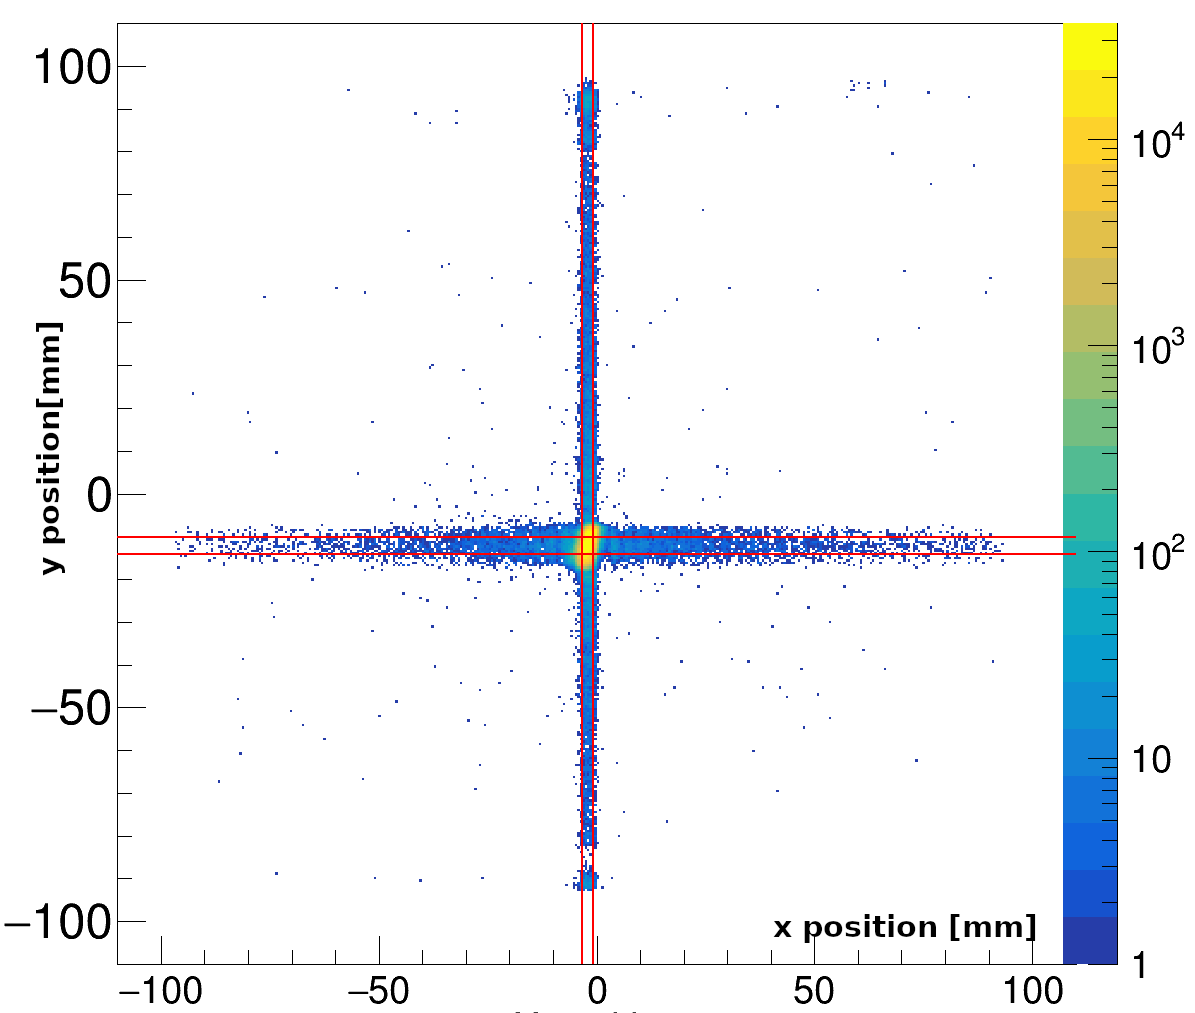
\includegraphics[width=\textwidth,keepaspectratio=true]{Figures/mw_no_cut.png}
  \caption{\textit{cal-to-hit} only. Events within $\pm1\sigma$: 901298}
  \label{fig:sub-first}
\end{subfigure}
\begin{subfigure}{.45\textwidth}
  \centering
  % include second image
  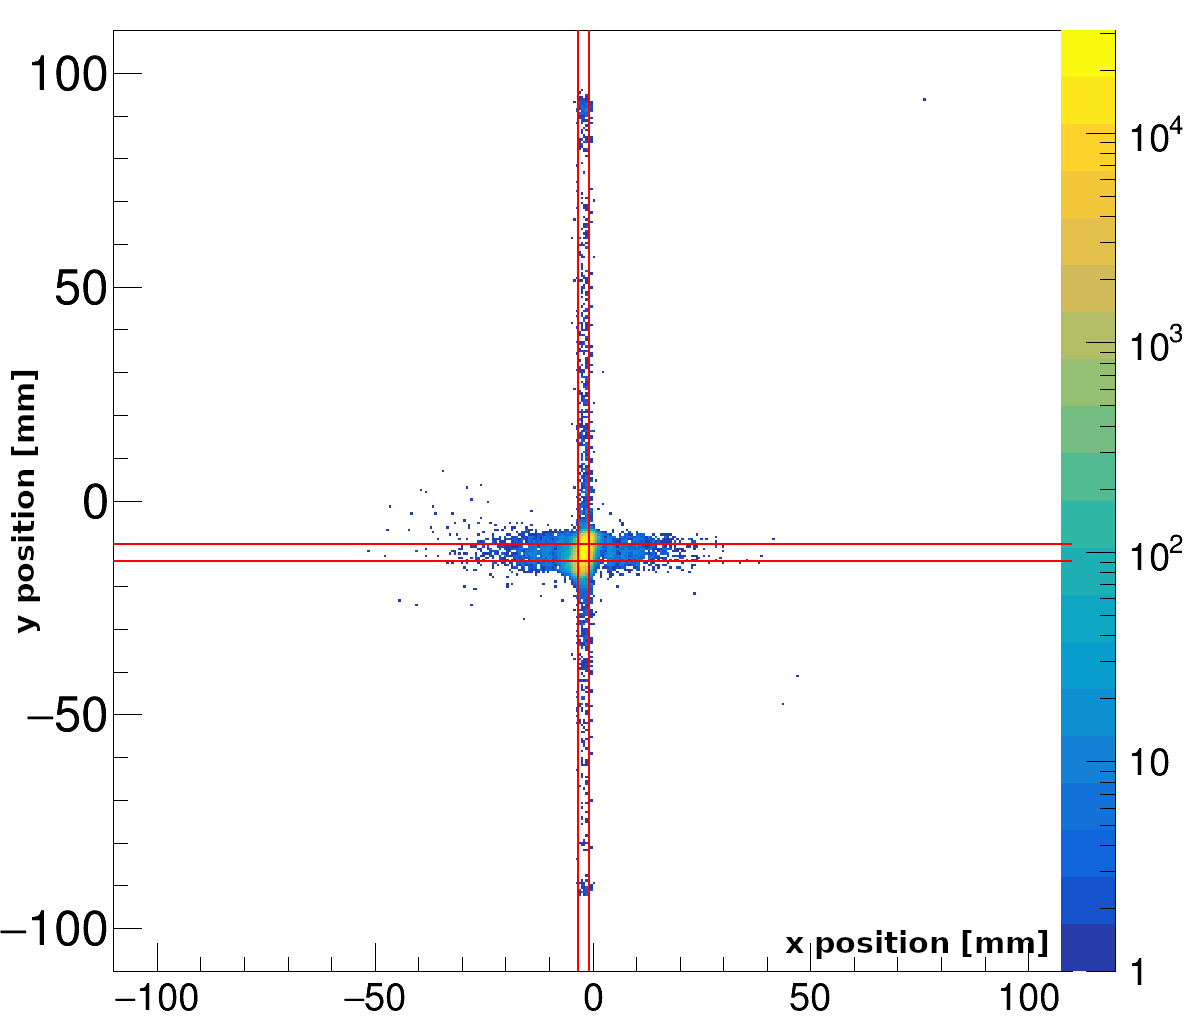
\includegraphics[width=\textwidth,keepaspectratio=true]{Figures/mw_coherent.png}
  \caption{Coherent clustering. Events within $\pm1\sigma$: 716002}
  \label{fig:sub-second}
\end{subfigure}

\begin{subfigure}{.45\textwidth}
  \centering
  % include third image
  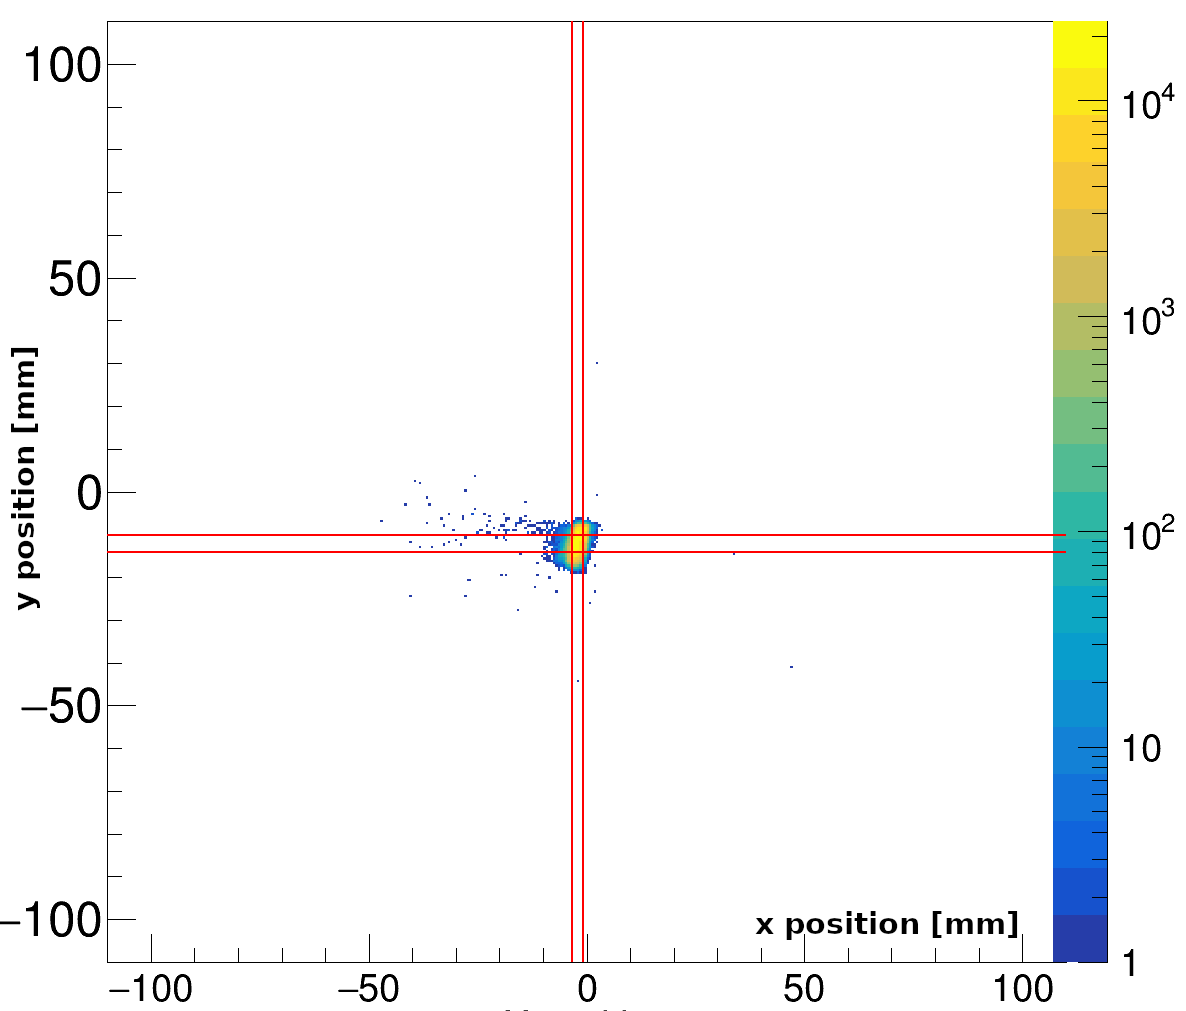
\includegraphics[width=\textwidth,keepaspectratio=true]{Figures/mw_coherent_less5.png}
  \caption{Coherent clustering \& less than 5 hits in x \& y. Events within $\pm1\sigma$: 514124}
  \label{fig:sub-third}
\end{subfigure}
\begin{subfigure}{.45\textwidth}
  \centering
  % include fourth image
  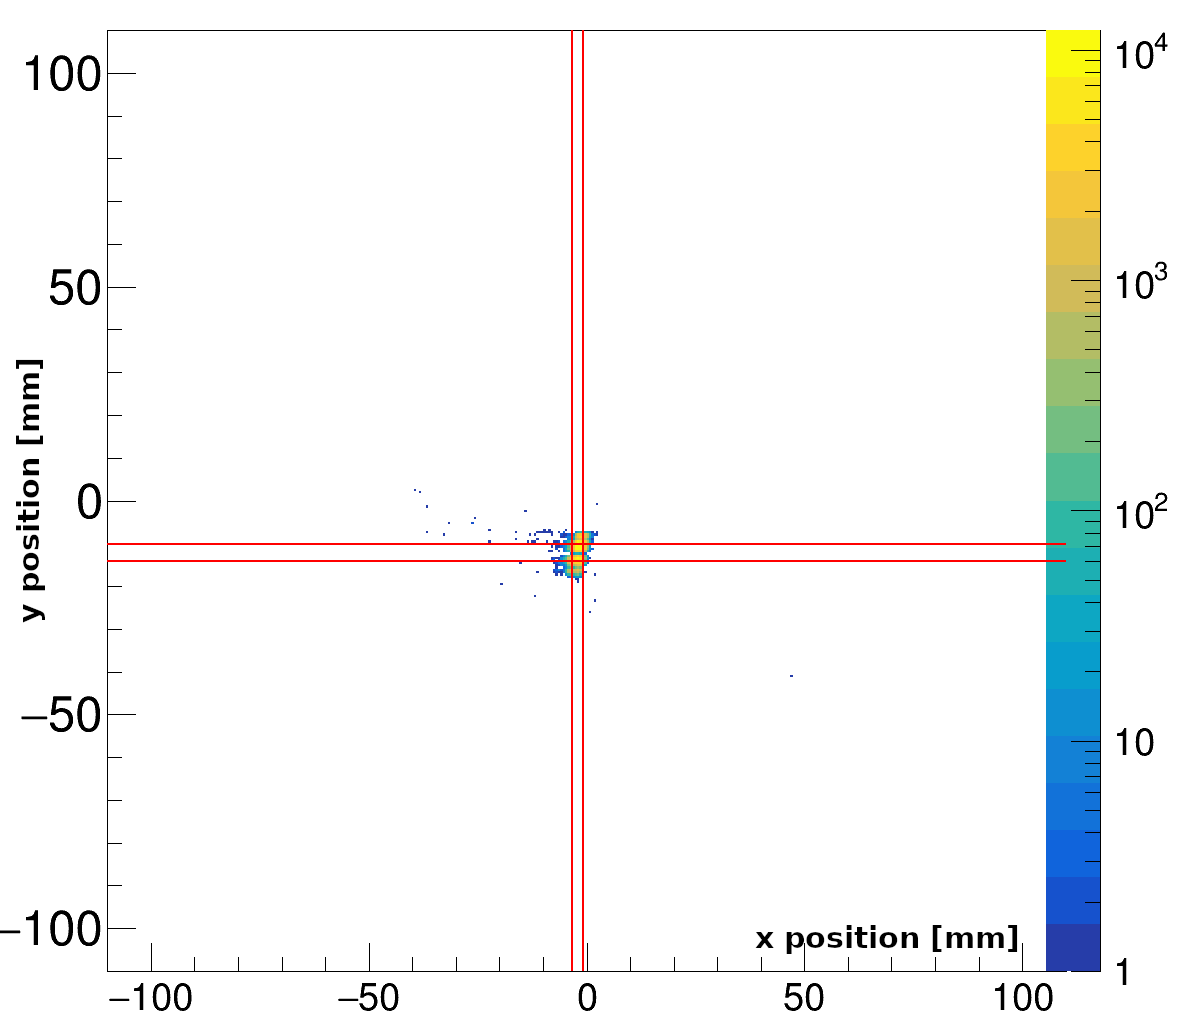
\includegraphics[width=\textwidth,keepaspectratio=true]{Figures/mw_coherent_less4.png}
  \caption{Coherent clustering \& less than 4 hits in x \& y. Events within $\pm1\sigma$\protect\footnotemark: 165144}
  \label{fig:sub-fourth}
\end{subfigure}
\caption{Overview of methods and cuts to clean up x \& y distibution on MWPC0 from misreconstruction.}
\label{fig:mw0_approaches}
\end{figure}
\footnotetext{The ripples in the y-reconstruction reflect the dimension of the readout pads in y-direction}
The effectiveness of these approaches is illustrated in Fig.~\ref{fig:mw0_approaches}. While both methods,when combined, significantly reduce the number of misreconstructed events and improve the spatial hit distribution, they lead to a substantial loss in statistics of more than 40\% (for coherent clustering \& less than 5 hits in x \& y).\newline
Since the $\pm1\sigma$ position cuts were already chosen to be sufficiently tight for the analysis, no additional selection criteria were applied for the MWPC0 event selection.


\section {Alternative methods for TWIN MUSIC hit selection and charge assignment} \label{app:twin_alternative}

\section {TWIN MUSIC Geometric Acceptance Correction via Efficiency Measurement}
Instead of correcting the limited geometric acceptance of TWIN MUSIC via graphical fitting (see section \ref{sec:geo_corr}) it is also feasible correcting via TWIN MUSIC efficiency measurement. The correction factor is given by:
\begin{equation}\label{eq:twin_eff}
\epsilon_{geo\text{\_}corr} = \frac{N_{MWPC1,MWPC2}}{N_{MWPC1,MWPC2,TWIN}}
\end{equation}
where $N_{MWPC1,MWPC2}$ corresponds to the number of events with a hit in MWPC1 and MWPC2 whereas $N_{MWPC1,MWPC2,TWIN}$ imposes the further condition having a hit in TWIN MUSIC too.\newline
The corresponding correction factor $\epsilon_{geo\text{\_}corr}$ is consequently applied on all target and empty runs. The resulting corrected charge changing cross section is shown in figure \ref{fig:twim_corr_cc_cs}. 
\begin{figure}[h!]
    \centering
    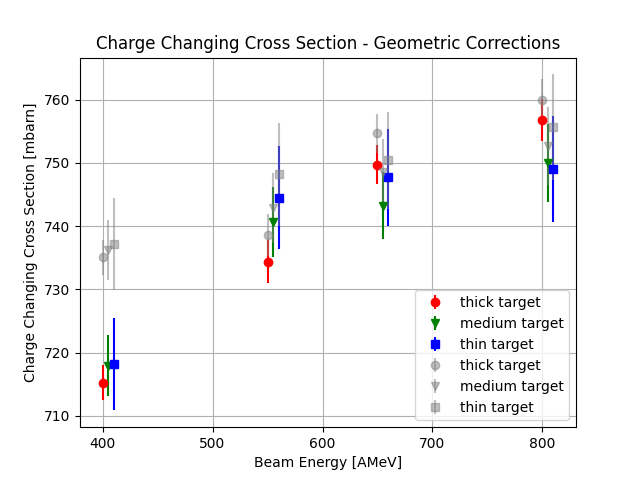
\includegraphics[width=\textwidth,height=8cm,keepaspectratio=true]{Figures/charge_changing_cross_sec_twim_eff_corr.png}
    \caption{
        Charge changing cross section correction due to limited geometric acceptance of TWIN MUSIC via efficiency correction with MWPC1 and MWPC2. In gray: charge changing cross section measurements before applying corrections, as in figure \ref{fig:cccs_gaus_diff_sections}}
    \label{fig:twim_corr_cc_cs}
\end{figure}
The same correction factor can be applied to the total interaction cross section as in figure \ref{fig:twim_corr_tot_cs}. 
\begin{figure}[h!]
    \centering
    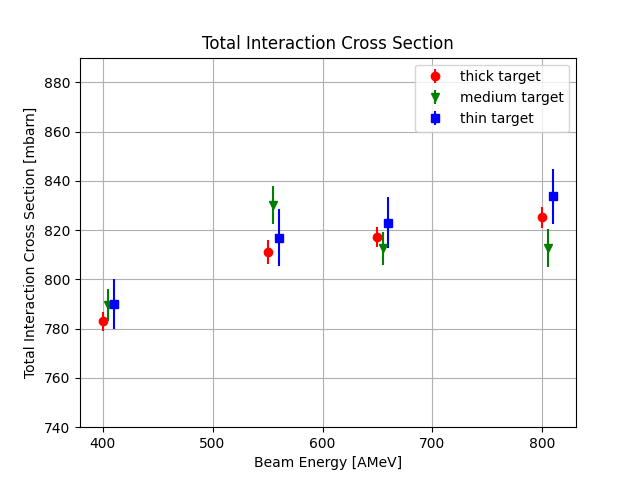
\includegraphics[width=\textwidth,height=12cm,keepaspectratio=true]{Figures/tot_interaction_cs_twim_eff_corr.png}
    \caption{
        Total interaction cross section of $^{12}$C + $^{12}$C using the TWIN MUSIC efficiency correction factor, see equation \ref{eq:twin_eff}, to compensate for the limited geometric acceptance in TWIN MUSIC.}
    \label{fig:twim_corr_tot_cs}
\end{figure}
\newpage



\section {Overview of isotope correction methods - selection cuts on the MWPC1/2/3}

\section{Flight-Path Reconstruction}\label{app:flightpath}
\begin{figure}[h!]
    \centering
    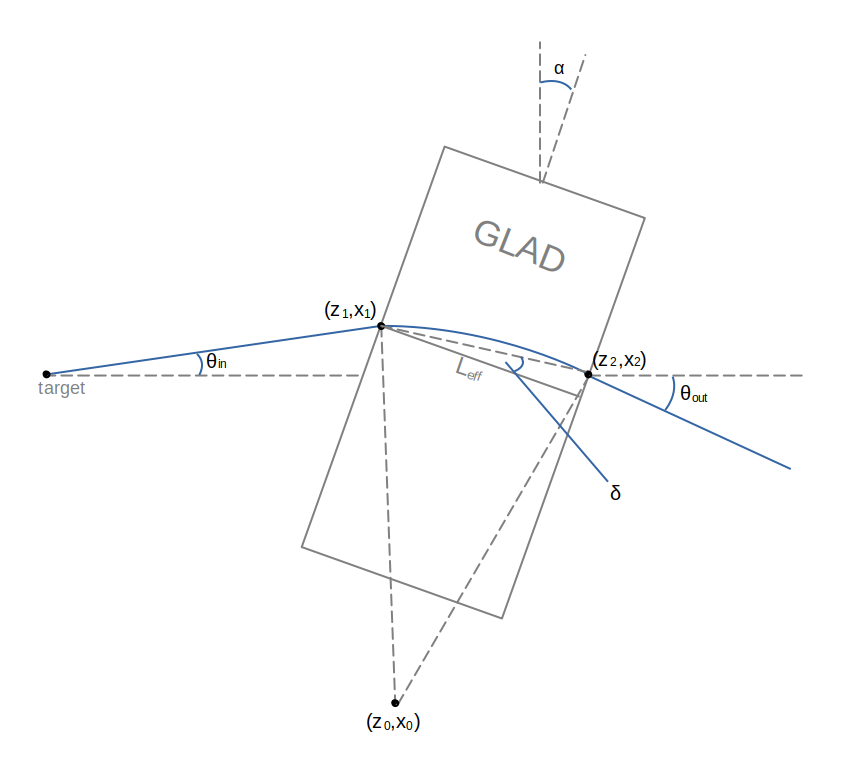
\includegraphics[width=\textwidth]{Figures/drawings_flightpath.png}
    \caption{
        Flightpath reconstruction with reference positions $(z_0,x_0)$, $(z_1,x_1)$ and $(z_2,x_2)$. The GLAD magnet is tilted by $\alpha = 14^{\circ}$.}
    \label{fig:draw_flight}
\end{figure}
The first step in the radius and flightpath reconstruction is expressing the entrance point on the GLAD field $(z_1,x_1)$ and the exit point $(z_2,x_2)$ with the center of the circle path $(z_0,x_0)$ as reference, see figure \ref{fig:draw_flight}:
\begin{align*}
z_1 &= z_0 -r\,cos(90^{\circ}-\theta_i) = z_0 -r\,sin(\theta_i)\\
x_1 &= x_0 + r\,sin(90^{\circ}-\theta_i) = x_0 + r\,cos(\theta_i)\\
\hspace{1cm}
z_2 &= z_0 + r\,cos(90^{\circ}-\theta_o) = z_0 + r\,sin(\theta_o)\\
x_2 &= x_0 + r\,sin(90^{\circ}-\theta_o) = x_0 + r\,cos(\theta_o) 
\end{align*}
The slope $m_1$ of the intersection line between $(z_1,x_1)$ and $(z_2,x_2)$ is given by:
\begin{align*}
m_1 &= \frac{x_2-x_1}{z_2 -z_1} = \frac{cos(\theta_o) - cos(\theta_i)}{sin(\theta_o)+sin(\theta_i)}
\end{align*}
and with the distance between the two points given by:
\begin{align*}
\Delta^2_{i/o} &= r^2 \, \left[(cos\theta_o - cos\theta_i)^2 + (sin\theta_o + sin\theta_i)^2 \right]\\
	       &= 4r^2\,sin^2(\frac{\theta_i}{2} +\frac{\theta_o}{2} )\\
\Rightarrow \Delta_{i/o} &= 2r\,sin(\frac{\theta_i}{2} +\frac{\theta_o}{2})
\end{align*}
To describe the distance between $(z_1,x_1)$ and $(z_2,x_2)$ with the given effective GLAD length $L_{eff}$ ($= 2.06\,m$) the tilting angle $\alpha$ (see figure \ref{fig:draw_flight}) of GLAD in relation to the incoming beam line direction has to be considered. Consequential the angle $\delta$ between the trajectory connecting $(z_1,x_1)$ and $(z_2,x_2)$ and the line parallel to the GLAD magnet width $L_{eff}$ can be determined as:
\begin{flalign*}
tan(\delta) &= \left| \frac{m_1-m_2}{1+ m_1\cdot m_2} \right|
\end{flalign*}
with $m_2 = -tan(\alpha)$:
\begin{align*}
\delta = atan \left( \frac{\frac{cos\theta_o - cos\theta_i}{sin\theta_o + sin\theta_i} + tan\alpha}{1-\frac{cos\theta_o - cos\theta_i}{sin\theta_o + sin\theta_i}\,\cdot\, tan\alpha} \right)
\end{align*}
The final relation between $L_{eff}$ and the bending radius $r$ of the fragment within GLAD can be written as:
\begin{equation}
\begin{aligned}
L_{eff} &= 2r\,sin(\frac{\theta_i}{2} + \frac{\theta_o}{2})\,\cdot\, cos\delta \\
	&= 2r\,sin(\frac{\theta_i}{2} + \frac{\theta_o}{2})\,\cdot\,\frac{1}{\sqrt{\delta^2+1}}
\end{aligned}
\end{equation}

\end{appendices}
